%!TEX root = nips2015.tex
\section{Experiments}
There are three major parameters in our system:
\\
1. Input representation of the game:
\\
We evaluated three different matrix representations of the Go board.
\\
i. One channel representation: Translating the board to a matrix directly by encoding a white stone as 255, a black stone as 0 and an empty position as 127. This was nearest to the Atari representation.
\\ii. Three channel representation: The first and second channels encode black and white stones respectively by placing a one in the matrix if there is a stone, 0 otherwise. The third channel places a one if there is a stone, zero if it is empty; this is basically the sum of first two channels.
\\
iii. Seven channel representation: This is inspired from Clark \& Storkey's input to the CNN which encodes information about the game itself by using the concept of liberties. A stone is said to have four liberties if the position to its left and right, top and bottom are empty, three if one of these positions is occupied by a competing stone and so on. The bottom left corner of Figure 1 shows a black stone with 2 liberties as it is surrounded by white on the left and top. If two stones of the same color are adjacent the liberties of each stone increases; this is depicted in the top left corner of Figure 1, where the group of three stones have a liberty count of 7. The diagonally placed stone has a liberty of four and is not part of the group. In this representation, we encode black positions in the first three channels by placing a one in the first channel if that stone has more than three liberties, one in the second channel if that stone has two, and one in the last channel if that stone has one liberty. The next three channels similarly encode positions of white stones. Each channel has a padding of three on either sides, so each channel of a 7 x 7 board will be of size 10 x 10. For the first six channels the padding is set to 0, whereas the seventh channel is 0 everywhere except at the padding where it is set to 1. This padding encodes the board's boundary.
\\
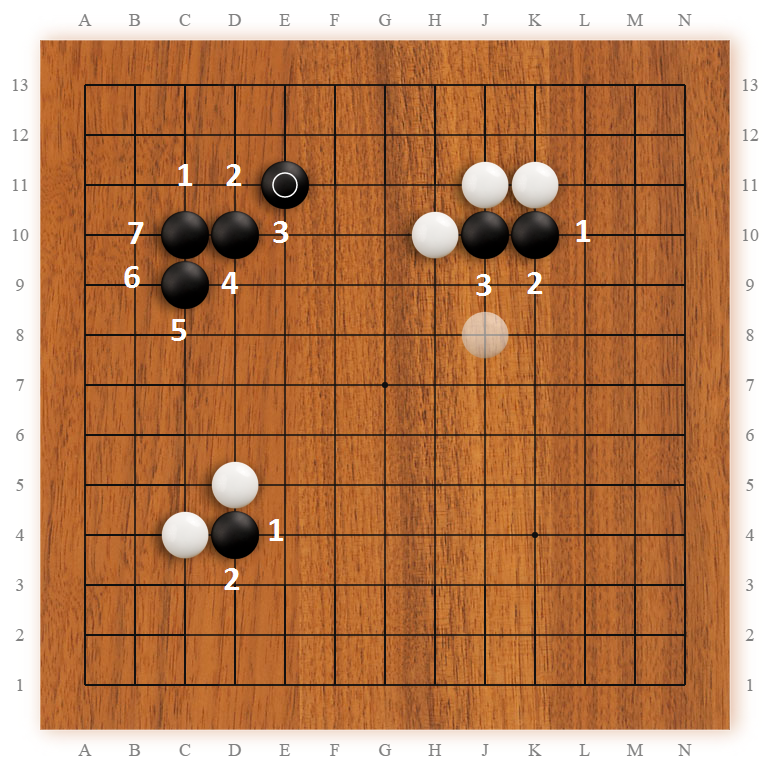
\includegraphics[scale=0.25]{ExampleLiberties}
\\
2. Architecture of the convolution neural network
\\
Briefly, the different network configurations we used are as follows:
\\
i. Two layer CNN with one dense layer and one softmax
\\
ii. Three layer CNN with one dense layer and one softmax
\\
iii. Five layer CNN with one dense layer
\\
iV. Seven layer CNN with one dense layer
\\
v. Five layer CNN with one dense layer and one multiplicative layer which zeroes out the q values of illegal moves
\\
In addition, we varied the filter sizes of the convolution layers.
\\
3. Parameters of Q Learning
\\
We varied the experience replay size and discount factor to find the right range of values. 
\\
